\documentclass[a4paper,12pt]{report}
\usepackage[utf8]{inputenc}
\usepackage{amsmath}
\usepackage{graphicx}
\usepackage{listings}
\usepackage{tikz}
\usepackage[T1]{fontenc}
\usepackage{color}
\usetikzlibrary{arrows,automata}
\definecolor{pythonred}{rgb}{0.6,0,0} % for strings
\definecolor{pythongreen}{rgb}{0.25,0.5,0.35} % comments
\definecolor{pythonpurple}{rgb}{0.5,0,0.35} % keywords
	\definecolor{pythondocblue}{rgb}{0.25,0.35,0.75} % javadoc
	 
	\lstset{language=python,
	basicstyle=\ttfamily,
	keywordstyle=\color{pythonpurple}\bfseries,
	stringstyle=\color{pythonred},
	commentstyle=\color{pythongreen},
	morecomment=[s][\color{pythondocblue}]{/**}{*/},
	numbers=left,
	numberstyle=\tiny\color{black},
        stepnumber=2,
	numbersep=10pt,
	tabsize=4,
	showspaces=false,
	showstringspaces=false}

% Title Page

 \title{\bfseries\huge \textcolor{purple}{\underline {EEP-703 Computer Network Lab}} \\{\textcolor{blue}{Assignment6-Simulate classical queueing models like M/M/1 Using Petri Net in SHARPE tool}}}
\author{\bfseries\large\textcolor{black}  {Harshit Kumar Gupta}\\ {\textcolor{black} {2013EET2369 }}\\

\includegraphics[width=3cm,height=3.4cm]{./iit.png}\\\noindent Computer Technology\\
\noindent Department Of Electrical Engineering\\IIT DELHI}
% iit.png: 282x282 pixel, 72dpi, 9.95x9.95 cm, bb=0 0 282 282
\begin{document}
\maketitle
\tableofcontents



\chapter{\textcolor{blue}{\underline {PROBLEM STATEMENT}}}
\noindent 

Consider a mail server of IIT Delhi with three departments have separate mail servers along
with an external mail server. The external mail server receives mails from all the three
department mail servers. Label the main server as node 0 and other three servers as node 1, 2
and 3. The messages, each with mean arrival rate 30 messages/sec arrive from three
department servers. The capacity of each duplex link is 100kb/sec with 5ms delay. Simulate
for 5 minutes to get the following performance measures. (consider M/M/1 queue between
the transmitting and the receiving nodes )

	
	\begin{enumerate}
	  \item Throughput at the central server (plot throughput versus simulation time).
	  \item  Plot queue length vs time and also calculate average queue length. (use monitor-queue
                 trace called qm.out)
	\end{enumerate}
	\noindent Compare the throughput at the central server when the queue size for all the links are changed
to 500 with that of default queue size provided in NS2. Give an explanation of the results
obtained. (M/M/1/K i.e. limited queue size)\\

\begin{center}
\chapter{\textcolor{blue}{\underline {ABSTRACT}}}
\end{center}
\noindent The SHARPE GUI implements eight interchangeable modeling description
techniques for reliability engineering: fault trees, Markov chains, reliability
block diagrams, reliability graphs, generalized stochastic Petri nets,
product queuing networks, multi-chain product form queuing networks
and task graphs. future, all the modeling description techniques contained
in SHARPE will be available in the GUI (phase mission, multi-components
fault trees, semi-Markov chains).
\begin{center}
\chapter{\textcolor{blue}{\underline {INTRODUCTION}}}
\end{center}
\noindent \textbf A Petri net (also known as a place/transition net or P/T net) is one of several mathematical 
modeling languages for the description of distributed systems. A Petri net is a directed bipartite graph, 
in which the nodes represent transitions (i.e. events that may occur, signified by bars) and places 
(i.e. conditions, signified by circles). The directed arcs describe which places are pre- and/or 
postconditions for which transitions (signified by arrows).\\

   Petri nets offer a graphical notation for stepwise processes that include choice, iteration, 
and concurrent execution. Unlike these standards, Petri nets have an exact mathematical definition
of their execution semantics, with a well-developed mathematical theory for process analysis.\\

The SHARPE GUI implements eight interchangeable modeling description
techniques for reliability engineering: fault trees, Markov chains, reliability
block diagrams, reliability graphs, generalized stochastic Petri nets,
product queuing networks, multi-chain product form queuing networks
and task graphs. future, all the modeling description techniques contained
in SHARPE will be available in the GUI (phase mission, multi-components
fault trees, semi-Markov chains).

\begin{center}
\chapter{\textcolor{blue}{\underline {SPECIFICATIONS AND ASSUMPTIONS}}}
\end{center}
\section*{Specifications}
\begin{enumerate}
 

 \item M/M/1 Queue and M/M/1-K Queue are used as queueing models
 \item Constant bit rate to be taken is 100kbps and lamda=30, mue=33.
 \item Perfomance Comparison has to be done with the help of THROUGHPUT.
\end{enumerate}

\section*{Assumptions}
\begin{enumerate}
\item Arrival rate propotional to tha packet size.
\item Virtual load will be propotional to the square of the arrival rate.
\item Other throughput degradation factors have been ignored.
\item Processing was taking long time to run therefore queue length is minimized.
\end{enumerate}
 
\begin{center}
\chapter{\textcolor{blue}{\underline {LOGIC USED/METHODOLOGY}}}
\end{center}
The methodology that is used for developing this project work is defined below:
\begin{enumerate} 
\item The entire code is drawn in rgl file format uisng Sharpe-GUI.
\item First, all the required 4 nodes are created in which node 0 acts as main server and node 1, 2, 3 are the departmental servers.
\item The tokens are created by using timed transitions with appropriate rate of generation.
\item The main server was connected to the three servers using untimed transitions.
\item The queue length was implemented using the inhibitor arc from a node to transition.
\item The various analysis graph and value were computed using the analysis tab in the menu of the Sharpe tool.
\item The required parameters were plotted.
\end{enumerate}

\begin{center}
\chapter{\textcolor{blue}{\underline {RESULTS AND CONCLUSIONS}}}\end{center}
\noindent The queueing models are designed as per the given requirements, and the simulation is working perfectly. The Graph Plotted studies the behaviour of Network under 
	  the M/M/1 queue model.
\begin{center}
Petri Net Model:
 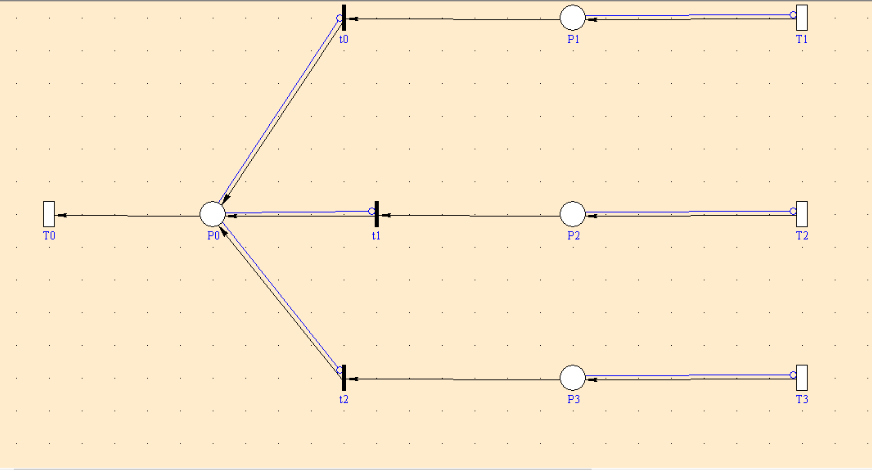
\includegraphics[width=13 cm,height=12 cm]{./assign6.PNG}
 % assign6.png: 1366x768 pixel, 96dpi, 36.15x20.32 cm, bb=0 0 1025 576
\end{center}

\begin{center}
Throughput Graph
 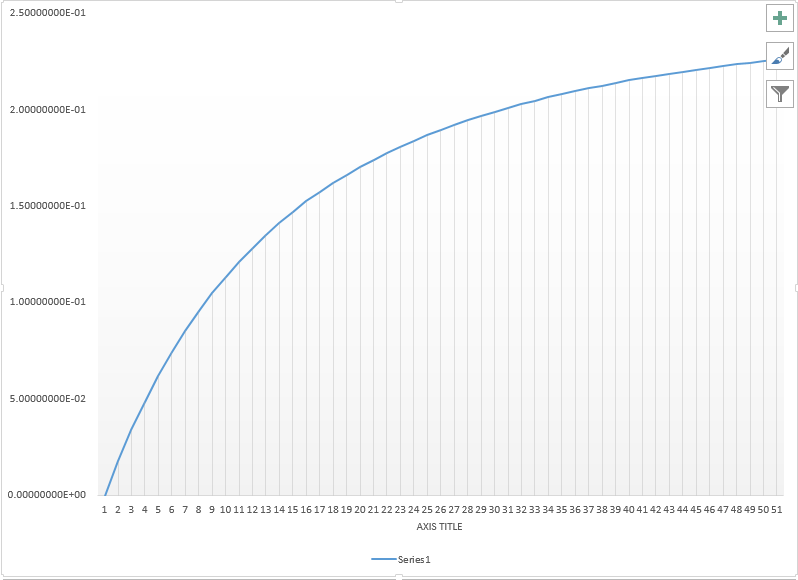
\includegraphics[width=15 cm,height=13 cm]{./throughput.PNG}
 % throughput.png: 1366x768 pixel, 96dpi, 36.15x20.32 cm, bb=0 0 1025 576
\end{center}
\begin{center}
QueueLength vs Time Graph
 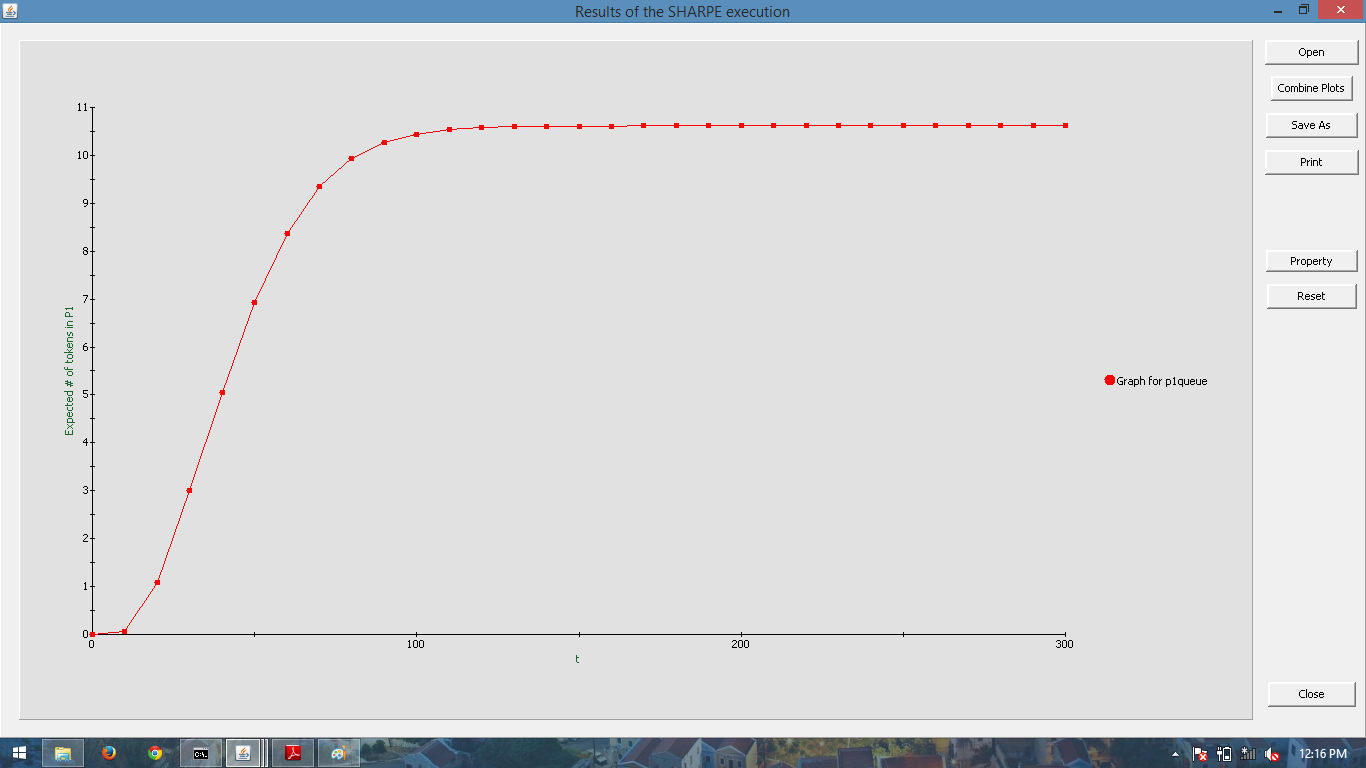
\includegraphics[width=15 cm,height=13 cm]{./queue1.png}
 % throughput.png: 1366x768 pixel, 96dpi, 36.15x20.32 cm, bb=0 0 1025 576
\end{center}

\begin{center}
Avg Queue Length at Central Server Graph
 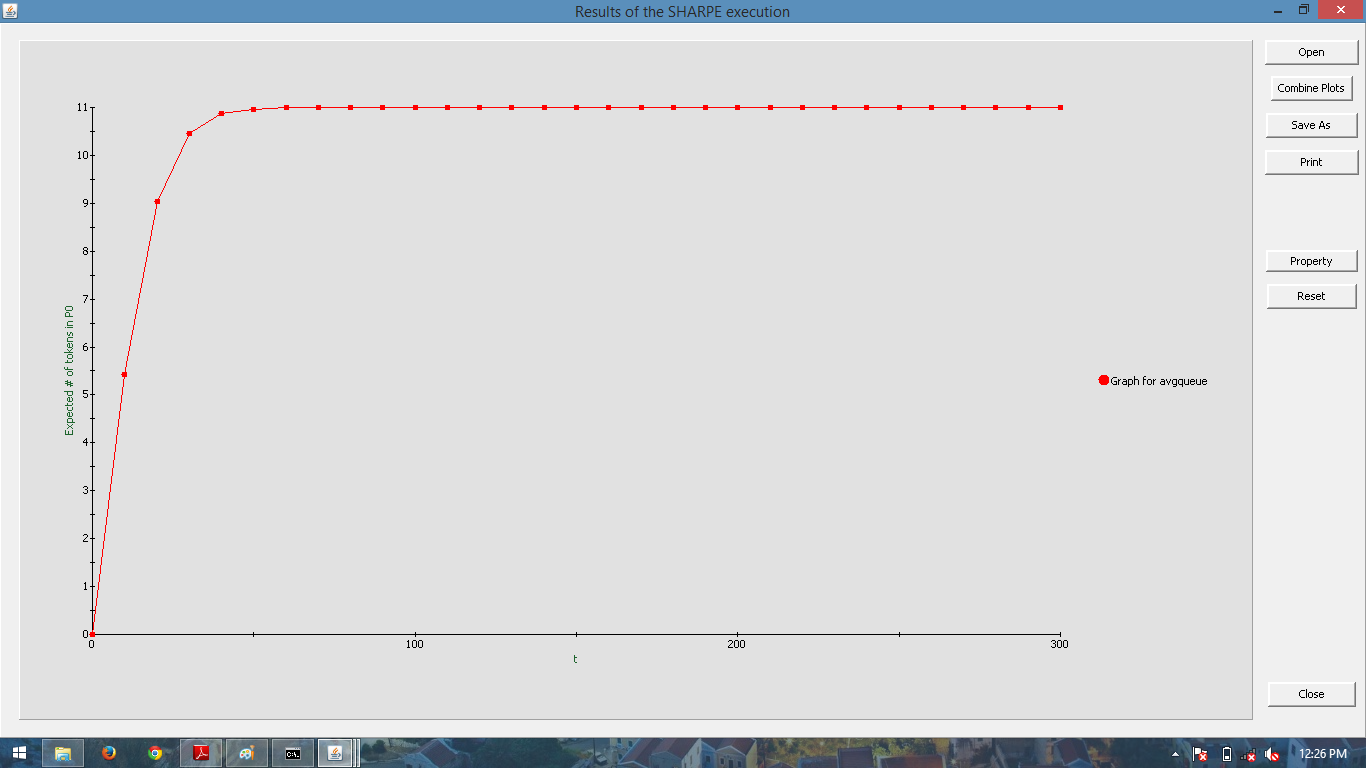
\includegraphics[width=15 cm,height=13 cm]{./queue.png}
 % throughput.png: 1366x768 pixel, 96dpi, 36.15x20.32 cm, bb=0 0 1025 576
\end{center}




\end{document}  